%% Font size %%
\documentclass[11pt]{article}

%% Load the custom package
\usepackage{Mathdoc}

%% Numéro de séquence %% Titre de la séquence %%
\renewcommand{\centerhead}{Chap. 4 : Tableau de variation}

%% Spacing commands %%
\renewcommand{\baselinestretch}{1}
\setlength{\parindent}{0pt}

\begin{document}

\begin{exercice}[0][Exercice corrigé.]
Dresser le tableau de signes de la fonction $f$ définie sur  $\mathbb
R$ par : $f(x)=-4x^2+16x+20$, sachant que $x_1=5$ et $x_2=-1$. \\
Ici, $a=-4$, donc la fonction est "en forme de cloche", elle est
\underline{négative} puis \underline{positive} et enfin \underline{négative}. \\
Donc le tableau de signes de $f$ sur $\mathbb{R}$  est :
\begin{center}
\begin{tikzpicture}[baseline, scale=0.75]
\tkzTabInit[lgt=3,deltacl=0.8,espcl=2.1]{ $x$ / 1.5, $f(x)$ / 1.5}{
  $-\infty$, $-1$, $5$, $+\infty$} \tkzTabLine{ , -, z, +, z, -}
\end{tikzpicture}
\end{center}
\end{exercice}

\end{document}
